\documentclass[11pt,a4paper]{article}
\usepackage[margin=2.5cm]{geometry}
\usepackage{booktabs}
\usepackage{hyperref}
\usepackage{graphicx}
\usepackage{amsmath}
\usepackage{listings}
\usepackage{xcolor}
\usepackage{microtype}
\usepackage{parskip}
\usepackage{caption}

\hypersetup{colorlinks=true, linkcolor=blue, urlcolor=blue, citecolor=blue}

\lstset{
  basicstyle=\ttfamily\small,
  backgroundcolor=\color{gray!8},
  frame=single,
  framerule=0.4pt,
  breaklines=true,
  breakatwhitespace=true,
  columns=flexible,
}

\title{\textbf{Audio Attribution}\\\large Final System: Top-K MERT k=10}
\author{Nikolaos Ballas}
\date{April 2026}

\begin{document}
\maketitle

\begin{quote}
\small\itshape
Disclaimer: Anthropic Claude was used as an engineering assistant for editing,
restructuring, and presentation support. The solution design, experimentation,
analysis, and final technical decisions are my own.
\end{quote}

% ─── Abstract ────────────────────────────────────────────────────────────────
\begin{abstract}
This report describes an audio attribution system that determines whether one
audio track is a derivative of another. The submitted system uses
\textbf{Top-K MERT k=10}: position-agnostic segment matching on MERT-v1-95M
embeddings, achieving ROC AUC \textbf{0.850} on the SONICS AI-generated audio
attribution benchmark. The approach requires no learned parameters beyond the
pre-trained MERT backbone and outperforms the best trained Siamese model
(ROC AUC 0.838 on MIPPIA) without any task-specific training.
\end{abstract}

% ─── 1. Task and Datasets ────────────────────────────────────────────────────
\section{Task and Datasets}

The task is pairwise attribution: given two audio tracks, return a score in
$[0,1]$ indicating how likely one is a derivative of the other, plus a
human-readable verdict.

\paragraph{MIPPIA.}
A curated dataset of 57 annotated positive pairs (known derivatives: remakes,
covers, interpolations) and 99 negative pairs, drawn from music plagiarism
litigation and academic annotation. Features are 782-dimensional:
MERT (768) + Chroma (12) + HP ratio (1) + Spectral Flatness (1).

\paragraph{SONICS.}
200 base IDs from the SONICS benchmark (parts 01--02), each with one original
track and one AI-generated derivative (Suno or Udio), giving 400 tracks and
200 positive pairs. 80 additional negative pairs were constructed by pairing
non-matching base IDs. SONICS tests the harder problem: detecting AI
generators that reproduce the musical structure of a source without copying
its audio signal.

% ─── 2. Feature Extraction ───────────────────────────────────────────────────
\section{Feature Extraction}

All audio is processed at 24\,kHz in 10-second non-overlapping segments.
Four feature types were extracted:

\begin{description}
  \item[MERT (768-dim)] \texttt{m-a-p/MERT-v1-95M} transformer embeddings.
    Each 10s segment produces one 768-dim vector. MERT captures musical
    structure, timbre, and rhythmic patterns in a learned semantic space.
  \item[CLAP (512-dim)] LAION-CLAP audio--text embeddings. Added for
    experiments requiring richer semantic context (1294-dim feature set).
    Not used in the final system.
  \item[Chroma (12-dim)] Chromagram, mean-pooled per segment. Captures
    harmonic content.
  \item[HP ratio (1-dim)] Harmonic/Percussive energy ratio from HPSS, in
    dB scale. Generator acoustic fingerprint feature.
  \item[Spectral Flatness (1-dim)] Mean spectral flatness. Measures
    tonal-vs-noise balance. Strongest single distributional signal on SONICS
    (effect size $r = 0.714$, Mann--Whitney $p = 0.0005$).
\end{description}

The final system uses \textbf{MERT only} (768-dim per segment). Spectral
Flatness and HP ratio were found to improve banded-diagonal track-level
comparison but \emph{not} segment-level Top-K matching (constant per-track
scalars dilute per-segment cosine similarity when tiled).

% ─── 3. Exploration Summary ──────────────────────────────────────────────────
\section{Exploration Summary}

The development followed a structured progression across two domains.

\subsection{MIPPIA domain (human plagiarism)}

\paragraph{Baseline: Calibrated cosine.}
Banded diagonal mean cosine similarity on 782-dim features, calibrated with
MIPPIA bounds (lo=0.88, hi=0.99). ROC AUC 0.708. Interpretable gap between
positive (0.89--0.95) and negative (0.20--0.34) pairs.

\paragraph{Siamese MLP 782-dim.}
A shared-encoder Siamese network (782$\to$512$\to$256) trained on 156 MIPPIA
positive pairs with pair-aware splitting. Mean ROC AUC \textbf{0.838} across
10 random seeds. Spectral Flatness (dim 781) had perturbation importance 0.491
--- dominant signal by a factor of 2.6$\times$ over all other dimensions.

\paragraph{1294-dim extensions.}
Adding CLAP (512-dim semantic embeddings) degraded MIPPIA performance to AUC
0.739 due to domain mismatch: CLAP penalises style dissimilarity even when
two tracks share composition but not genre. Hard-negative mining further
degraded to AUC 0.635 --- the 57-pair MIPPIA dataset is too small for hard
negatives to be outside the positive cluster.

\paragraph{Calibration failure on SONICS.}
The MIPPIA-calibrated system collapses on AI-generated pairs: both positive
and negative pairs score $\approx 1.0000$ because MIPPIA calibration bounds
(lo=0.88, hi=0.99) are compressed far below the SONICS similarity
distribution (which sits above 0.92).

\subsection{SONICS domain (AI-generated attribution)}

\paragraph{Recalibration diagnosis.}
Fitting SONICS-specific bounds (lo=0.9220, hi=0.9336) from 200 base IDs
recovered the hidden signal. Banded diagonal cosine on MERT with SONICS
calibration: AUC 0.675. The signal was always present in MERT --- MIPPIA
calibration was masking it.

\paragraph{Generator artifact features.}
Spectral Flatness and HP ratio show dramatically stronger distributional
separation on SONICS than on MIPPIA:
Spectral Flatness effect size $r=0.714$ on SONICS vs $r=0.18$ on MIPPIA
($4\times$ stronger); HP ratio $r=0.700$ vs $r=0.38$ ($1.8\times$).
AI vocoders produce characteristic tonal-noise balance consistent within a
generator. Combined MERT+SF+HP: AUC 0.745. However, these are track-level
scalars (extracted from the first 30 seconds) and cannot be used at segment
level.

\paragraph{Adapter MLP.}
A small adapter (768$\to$128$\to$128, 131k parameters) trained on top of
frozen MERT on 640 SONICS pairs achieved AUC 0.498 --- below random. The
model overfits from epoch 2. The data threshold for a neural adapter to beat
cosine similarity is estimated at $\approx$5\,000 pairs (500+ base IDs);
the available 200 base IDs are insufficient.

\paragraph{Top-K: the key insight.}
The transition from banded diagonal (AUC 0.675) to Top-K (AUC 0.850) is the
central result. Banded diagonal assumes borrowed content appears at the
\emph{same relative timestamp} in both tracks. This assumption holds for
human remakes (temporal structure is preserved) but breaks for AI
attribution: generators reconstruct musical content without preserving
temporal position. Top-K segment matching finds the best-matching segment
\emph{anywhere in Track B} for each segment of Track A, removing the
temporal assumption.

% ─── 4. Final System ─────────────────────────────────────────────────────────
\section{Final System: Top-K MERT k=10}

\subsection{Algorithm}

\begin{enumerate}
  \item Extract MERT-v1-95M embeddings for each 10-second segment of both
    tracks, producing matrices $A \in \mathbb{R}^{N_A \times 768}$ and
    $B \in \mathbb{R}^{N_B \times 768}$.
  \item Compute the full cosine similarity matrix
    $S \in \mathbb{R}^{N_A \times N_B}$, normalised to $[0,1]$.
  \item For each row $i$ of $S$ (each segment of Track A), find
    $s_i = \max_j S_{ij}$ --- the most similar segment anywhere in Track B.
  \item Average the top-$k$ values of $\{s_1, \ldots, s_{N_A}\}$:
    \[
      \text{raw} = \frac{1}{k}\sum_{i \in \text{top-}k} s_i, \qquad k = 10.
    \]
  \item Calibrate to $[0,1]$ using SONICS distribution bounds:
    \[
      \text{score} = \text{clip}\!\left(\frac{\text{raw} - \text{lo}}
        {\text{hi} - \text{lo}},\; 0,\; 1\right),
      \quad \text{lo} = 0.9220,\; \text{hi} = 0.9336.
    \]
\end{enumerate}

Verdicts are assigned by score threshold: $\geq 0.75$ LIKELY DERIVATIVE,
$\geq 0.55$ POSSIBLY RELATED, $\geq 0.35$ WEAK SIMILARITY, otherwise UNRELATED.

\subsection{K-sweep validation}

\begin{table}[h]
\centering
\caption{ROC AUC vs.\ $k$ (Top-K MERT, SONICS, 200 base IDs).}
\begin{tabular}{lcccccc}
\toprule
$k$ & 1 & 3 & 5 & 10 & 20 & Banded diag. \\
\midrule
AUC & 0.839 & 0.846 & 0.843 & \textbf{0.850} & 0.845 & 0.749 \\
\bottomrule
\end{tabular}
\end{table}

The improvement is stable across $k$. $k=10$ is optimal and selected as the
submitted value. All Top-K variants substantially outperform banded diagonal
($+0.101$ at $k=10$).

\begin{figure}[h]
\centering
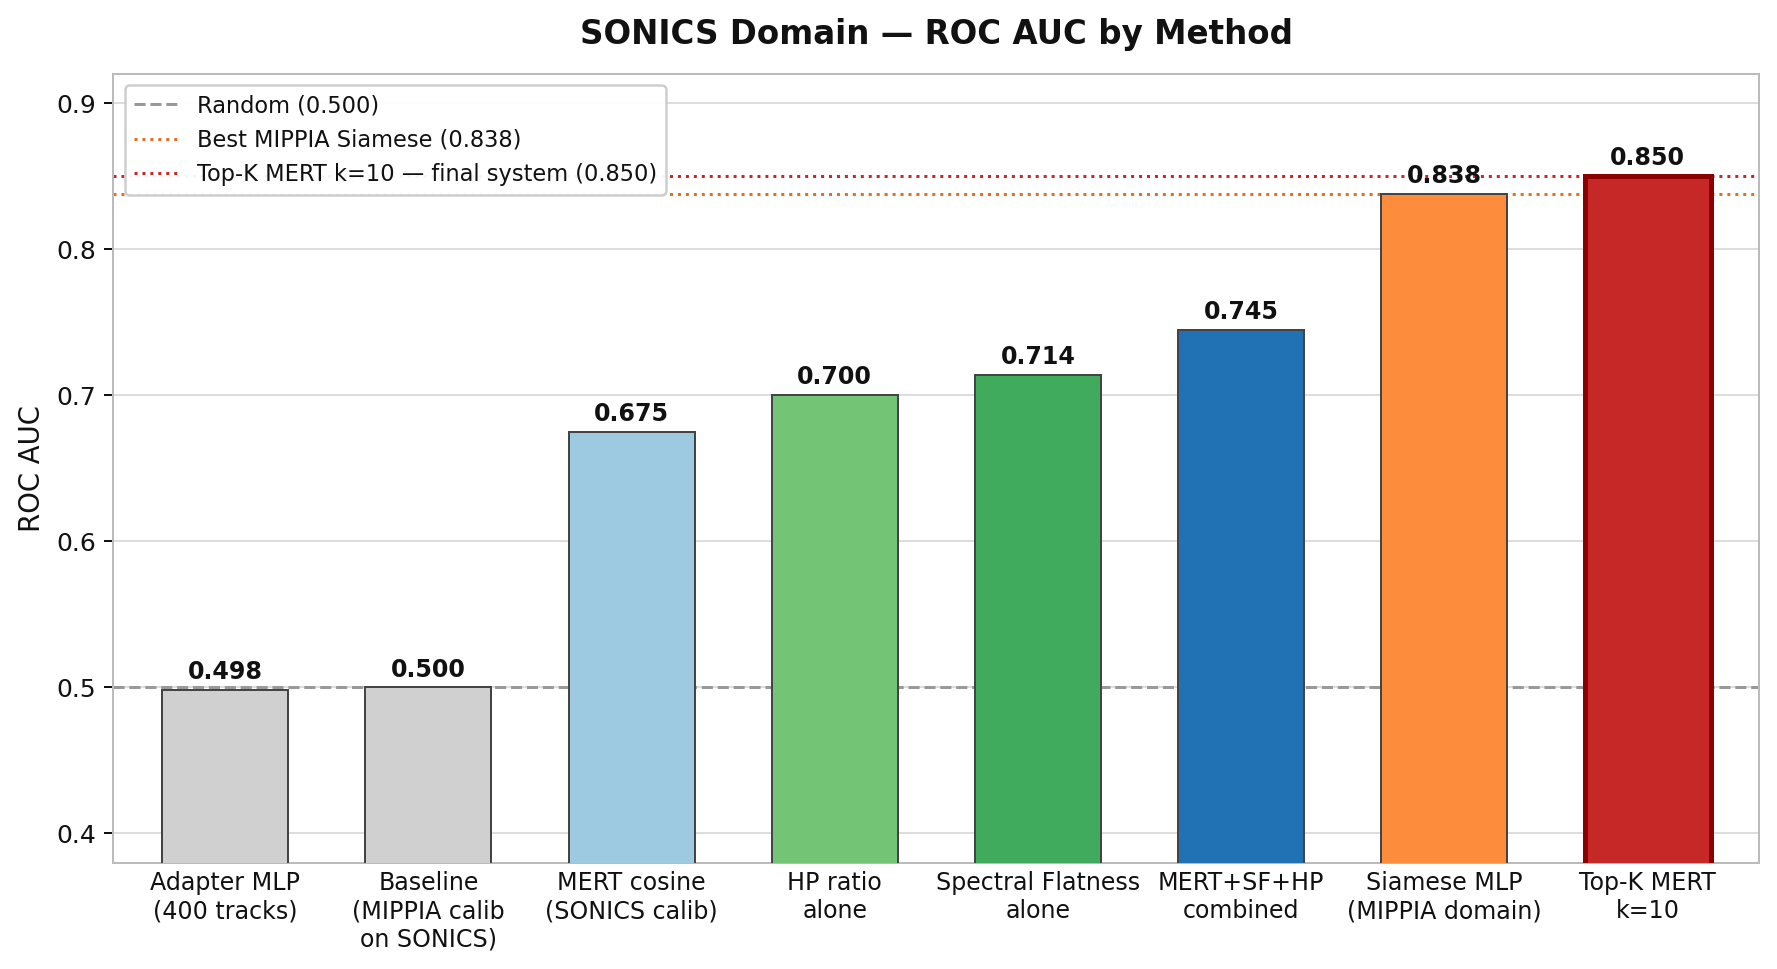
\includegraphics[width=0.7\textwidth]{../results/sonics/sonics_results.png}
\caption{ROC AUC by method on the SONICS domain. Top-K MERT k=10 (AUC 0.850,
highlighted in red) is the final submitted system and the best result overall.
Grey bars are non-competitive baselines; orange is the best MIPPIA result
shown for cross-domain reference.}
\end{figure}

\subsection{Comparison with other methods}

\begin{table}[h]
\centering
\caption{All methods evaluated on their respective test sets.}
\begin{tabular}{llll}
\toprule
Method & Domain & ROC AUC & Notes \\
\midrule
\textbf{Top-K MERT k=10} & \textbf{SONICS} & \textbf{0.850} & \textbf{Final system} \\
MERT + SF + HP combined & SONICS & 0.745 & Track-level only \\
Spectral Flatness alone & SONICS & 0.714 & Single scalar \\
HP ratio alone & SONICS & 0.700 & Single scalar \\
MERT cosine (SONICS calib.) & SONICS & 0.675 & Banded diagonal \\
Siamese MLP 782-dim & MIPPIA & 0.838 & Best on MIPPIA \\
Calibrated cosine (MIPPIA) & MIPPIA & 0.708 & Simple baseline \\
Adapter MLP (400 tracks) & SONICS & 0.498 & Insufficient data \\
\bottomrule
\end{tabular}
\end{table}

% ─── 5. Usage ────────────────────────────────────────────────────────────────
\section{Usage}

\subsection{Command-line interface}

\begin{lstlisting}
# Audio files
python compare_tracks.py track_a.mp3 track_b.mp3

# Pre-extracted demo features (no audio needed)
python compare_tracks.py demo/001_ori.npy demo/001_comp.npy
\end{lstlisting}

The script accepts audio files (\texttt{.mp3}, \texttt{.wav}, \texttt{.flac}) or
pre-extracted \texttt{.npy} feature files. On first run it creates a local venv
and installs dependencies. The included demo files produce:

\begin{lstlisting}
=================================================================
  Score:   1.0000  [????????????????????????????????????????????????]  100.0%
  Verdict: LIKELY DERIVATIVE
  Raw:     0.9644  (lo=0.9220  hi=0.9336)
  Method:  Top-K MERT k=10  (0.6s)
=================================================================
\end{lstlisting}

\subsection{Python API}

\begin{lstlisting}[language=Python]
from src.compare_tracks_api import compare_tracks, compare_tracks_from_paths

# By registered ID (src/registry.py)
result = compare_tracks("001_ori", "001_comp")
# {"score": 1.0, "verdict": "LIKELY DERIVATIVE", ...}

# By path
result = compare_tracks_from_paths("track_a.mp3", "track_b.mp3")
\end{lstlisting}

% ─── 6. Limitations ──────────────────────────────────────────────────────────
\section{Limitations}

\paragraph{Calibration scope.}
SONICS calibration bounds (lo=0.9220, hi=0.9336) were estimated from 200 base
IDs in SONICS parts 01--02, which contain single-generator pairs only (all
Suno or all Udio per base ID). Cross-generator attribution (detecting that a
Udio track is derived from a Suno original, or vice versa) is untested.
SONICS parts 03--10 would be needed to validate cross-generator performance.

\paragraph{Score saturation.}
Positive pairs in the provided demo score 1.0000 due to the narrow calibration
range. The raw MERT similarity (0.9644) is more informative in the upper tail.
Wider calibration windows, or reporting raw scores, would improve
discrimination between degrees of derivation.

\paragraph{FakeMusicCaps not used.}
The FakeMusicCaps dataset (10-second TTM clips) was not incorporated. Its
short clip length requires a different segmentation pipeline; given GPU and
time constraints it was deprioritised in favour of SONICS coverage.

\paragraph{Neural adapter data threshold.}
A trained adapter can be expected to outperform cosine similarity at
approximately 5\,000 pairs (500+ base IDs). The available SONICS data is
insufficient for this approach. Top-K MERT is the correct system for the
current data scale.

\paragraph{GPU for extraction.}
MERT extraction on CPU takes approximately 10 minutes per track. The included
\texttt{demo/*.npy} files bypass extraction entirely and allow instant
evaluation without GPU.

% ─── References ──────────────────────────────────────────────────────────────
\section*{References}

\begin{description}
  \item[MERT] Li et al., \textit{MERT: Acoustic Music Understanding Model
    with Large-Scale Self-Supervised Training}, ICLR 2024.
    \texttt{m-a-p/MERT-v1-95M}.
  \item[SONICS] \textit{SONICS: Synthetic Or Not --- Identifying Counterfeit
    Songs} benchmark, Hugging Face dataset.
  \item[MIPPIA] \textit{Music Information Processing for Plagiarism and
    Infringement Analysis} dataset, annotated music plagiarism pairs.
\end{description}

\end{document}
